\documentclass{beamer}

\mode<presentation>
{
   % \usetheme{CambridgeUS}
  \usetheme{Hannover}
  \setbeamercovered{invisible}
  \setbeamertemplate{navigation symbols}{\insertframenumber/\inserttotalframenumber}%replace navigation symbols
}

\usepackage[english]{babel}
\usepackage[latin1]{inputenc}
\usepackage{times}
\usepackage[T1]{fontenc} 
% Or whatever. Note that the encoding and the font should match. If T1
% does not look nice, try deleting the line with the fontenc.
% \usepackage{amsmath}
\usepackage{appendixnumberbeamer}

\newcommand{\linespace}{\vskip 0.25cm}

% The text in square brackets is the short version of your title and will be used in the
% header/footer depending on your theme.
\title{Automated Lineage Analysis\\for\\Evolved Programs}
%{Using Graph Databases to Explore Genetic Programming Run Dynamics}

% Sub-titles are optional - uncomment and edit the next line if you want one.
% \subtitle{[subtitle goes here if we want one]} 

% The text in square brackets is the short version of your name(s) and will be used in the
% header/footer depending on your theme.
% \author[Laverne Schrock]{Laverne Schrock w/ Nic Mcphee}
\author[Laverne Schrock]{Laverne Schrock}

% The text in square brackets is the short version of your institution and will be used in the
% header/footer depending on your theme.
% \institute[UMN Morris]
% {
%   Division of Science and Mathematics \\
%   University of Minnesota, Morris \\
%   Morris, Minnesota, USA \\
% }
% ^^ Probably want to cut this ?

% The text in square brackets is the short version of the date if you need that.
\date[June 2016] % (optional)
% {May 2016 \\ Genetic Programming Theory and Practice \\ University of Michigan \\ Ann Arbor, MI}

% Delete this, if you do not want the table of contents to pop up at
% the beginning of each subsection.
% \AtBeginSection[]
% {
%   \begin{frame}<beamer>
%     \frametitle{Outline}
%     \tableofcontents[currentsection, hideothersubsections]
%   \end{frame}
% }

\begin{document}

\begin{frame}
  \titlepage
\end{frame}

% For a 20-25 minute senior seminar talk you probably want something like:
% - Two or three major sections (other than the summary).
% - At *most* three subsections per section.
% - Talk about 30s to 2min per frame. So there should probably be between
%   15 and 30 frames, all told.

\subsection*{Outline}

\begin{frame}
  \frametitle{Outline}
  % \tableofcontents[hideallsubsections]
  \tableofcontents
\end{frame}


% \section{Overview}

% \subsection{The Big Picture}

% \begin{frame}
%   \frametitle{The Big Picture}
  
%   \begin{itemize}
% 	\item Genetic programming clearly \emph{works}.
% 	\item But we rarely know \emph{why} or \emph{how}.
% 	\item Databases allow examination of the internal interactions of a run.
% 	\item Graph databases allow us to collect and analyze lineages.
% 	\item Silico-paleontology can help us understand and improve our tools.
%   \end{itemize}

% \end{frame}

\section{Genetic Programming}
   \subsection{In General Terms}
   \begin{frame}
     \frametitle{Genetic Programming}
     \begin{itemize}
     \item Randomly create a bunch of programs
     \item Test each program's performance
     \item Use the better programs to create a new generation
     \item Repeat until...
     \item A program passes the tests perfectly \em or \em we give up
     \end{itemize}
   \end{frame}
% \begin{frame}[fragile]
%   \frametitle{Example Push Genome}
% \begin{verbatim}
% [{:instruction 1 :close 0}
%  {:instruction 2 :close 0}
%  {:instruction integer_add :close 0}
%  {:instruction 3 :close 0}
%  {:instruction exec_if :close 0}
%  {:instruction "equal" :close 0}
%  {:instruction "not equal" :close 0}]
% \end{verbatim}
% \end{frame}

   \begin{frame}
     \frametitle{Randomly create a bunch of programs}
     \begin{itemize}
     \item Primordial ooze
     \item Maximum size of 400 genes
     % \item Randomly create a bunch of programs
     \item 1000 individuals
       % Do I really want to talk about Lexicase
       % selection?  It is super cool, but we have limited time and I'm not sure
       % that it is very important to what I'm doing this summer.
     \end{itemize}
   \end{frame}
   % Question: I like the term ``evolutionary system''. Is this term ever used
   % in the field?

   \begin{frame}
     \frametitle{Test each program's performance}
     \begin{itemize}
     \item Expected outputs are provided
     \item An error of 0 is perfect
     \item The Replace Space with Newline problem has 200 tests
     \end{itemize}
   \end{frame}

   \begin{frame}
     \frametitle{Create a new generation}
     Creation Process
     \begin{itemize}
       \item Chose Genetic Operator 
       \item Select parent(s) 
       \item Apply operator to generate child
     \end{itemize}
     Genetic Operators
     \begin{itemize}
     \item Alternation (20\%)
     \item Uniform mutation (20\%)
     \item Uniform close mutation (10\%)
     \item Alternation followed by uniform mutation (50\%)
     \end{itemize} 
     % Which operations allow for deletions of genomes?
   \end{frame}

   \begin{frame}
    \frametitle{Termination} 
    \begin{itemize}
    \item When solution(s) are found
    \item Capped at 300 generations 
    \end{itemize}
   \end{frame}

   \subsection{Details regarding our specific evolutionary system}

   \begin{frame}
     \frametitle{Clojush}
     \begin{itemize}
     \item Clojure implementation of PushGP 
     \item Evolves Push programs
     \item Produces extensive logs
     % \item Linear Genome % I'll have to mention this at some point....???
     \end{itemize}
   \end{frame}


\begin{frame}[fragile]
\frametitle{Push Program}
\begin{overprint}
\onslide<1>
\begin{semiverbatim}
exec: (``AbcAbcAbc'' \char`\\A string\_removechar
        string\_length)
string: ()
character: ()
integer: ()
\end{semiverbatim}
\onslide<2>
\begin{semiverbatim}
exec: (\char`\\A string\_removechar string\_length)
string: (``AbcAbcAbc'')
character: ()
integer: ()
\end{semiverbatim}
\onslide<3>
\begin{semiverbatim}
exec: (string\_removechar string\_length)
string: (``AbcAbcAbc'')
character: (\char`\\A)
integer: ()
\end{semiverbatim}
\onslide<4>
\begin{semiverbatim}
exec: (string\_length)
string: (``bcbcbc'')
character: ()
integer: ()

\end{semiverbatim}
\onslide<5>
Final State:
\begin{semiverbatim}
exec: ()
string: ()
character: ()
integer: (6)
\end{semiverbatim}
Original Program:
\begin{semiverbatim}
exec: (``AbcAbcAbc'' \char`\\A string\_removechar
        string\_length)
\end{semiverbatim}
\end{overprint}
\end{frame}

   \section{Previous Work \& Motivation}
   \subsection{Storing the Data}
   \begin{frame}
     \frametitle{Storing the data}
   Information recorded for each individual:
   \begin{itemize}
   \item Parents
   \item Formation Method (Alternation, Mutation, ...)
   \item Genome
   \item Error Vector
   \end{itemize}
   This data takes a lot of space! 
   \begin{itemize}
   \item 2~TB of compressed data in Tom Helmuth's dataset
   \end{itemize}
   % Large amount of data to store. In a failed run, 300 generations $\times$ 1000
   % individuals = 300,000 individuals. Other types of problems may be allowed to
   % run for a few thousand generations.
   \end{frame}
   % \begin{frame}
   %   \frametitle{Why store the data?}
   %   \begin{itemize}
   %   \item Most researchers only collect aggregate statistics
   %   \item ,b
   %   \end{itemize}
   % \end{frame}
   \subsection{Full Analysis (spring 2016)}

   \begin{frame}
     \frametitle{Filtering - Full Ancestry}
     \centering
     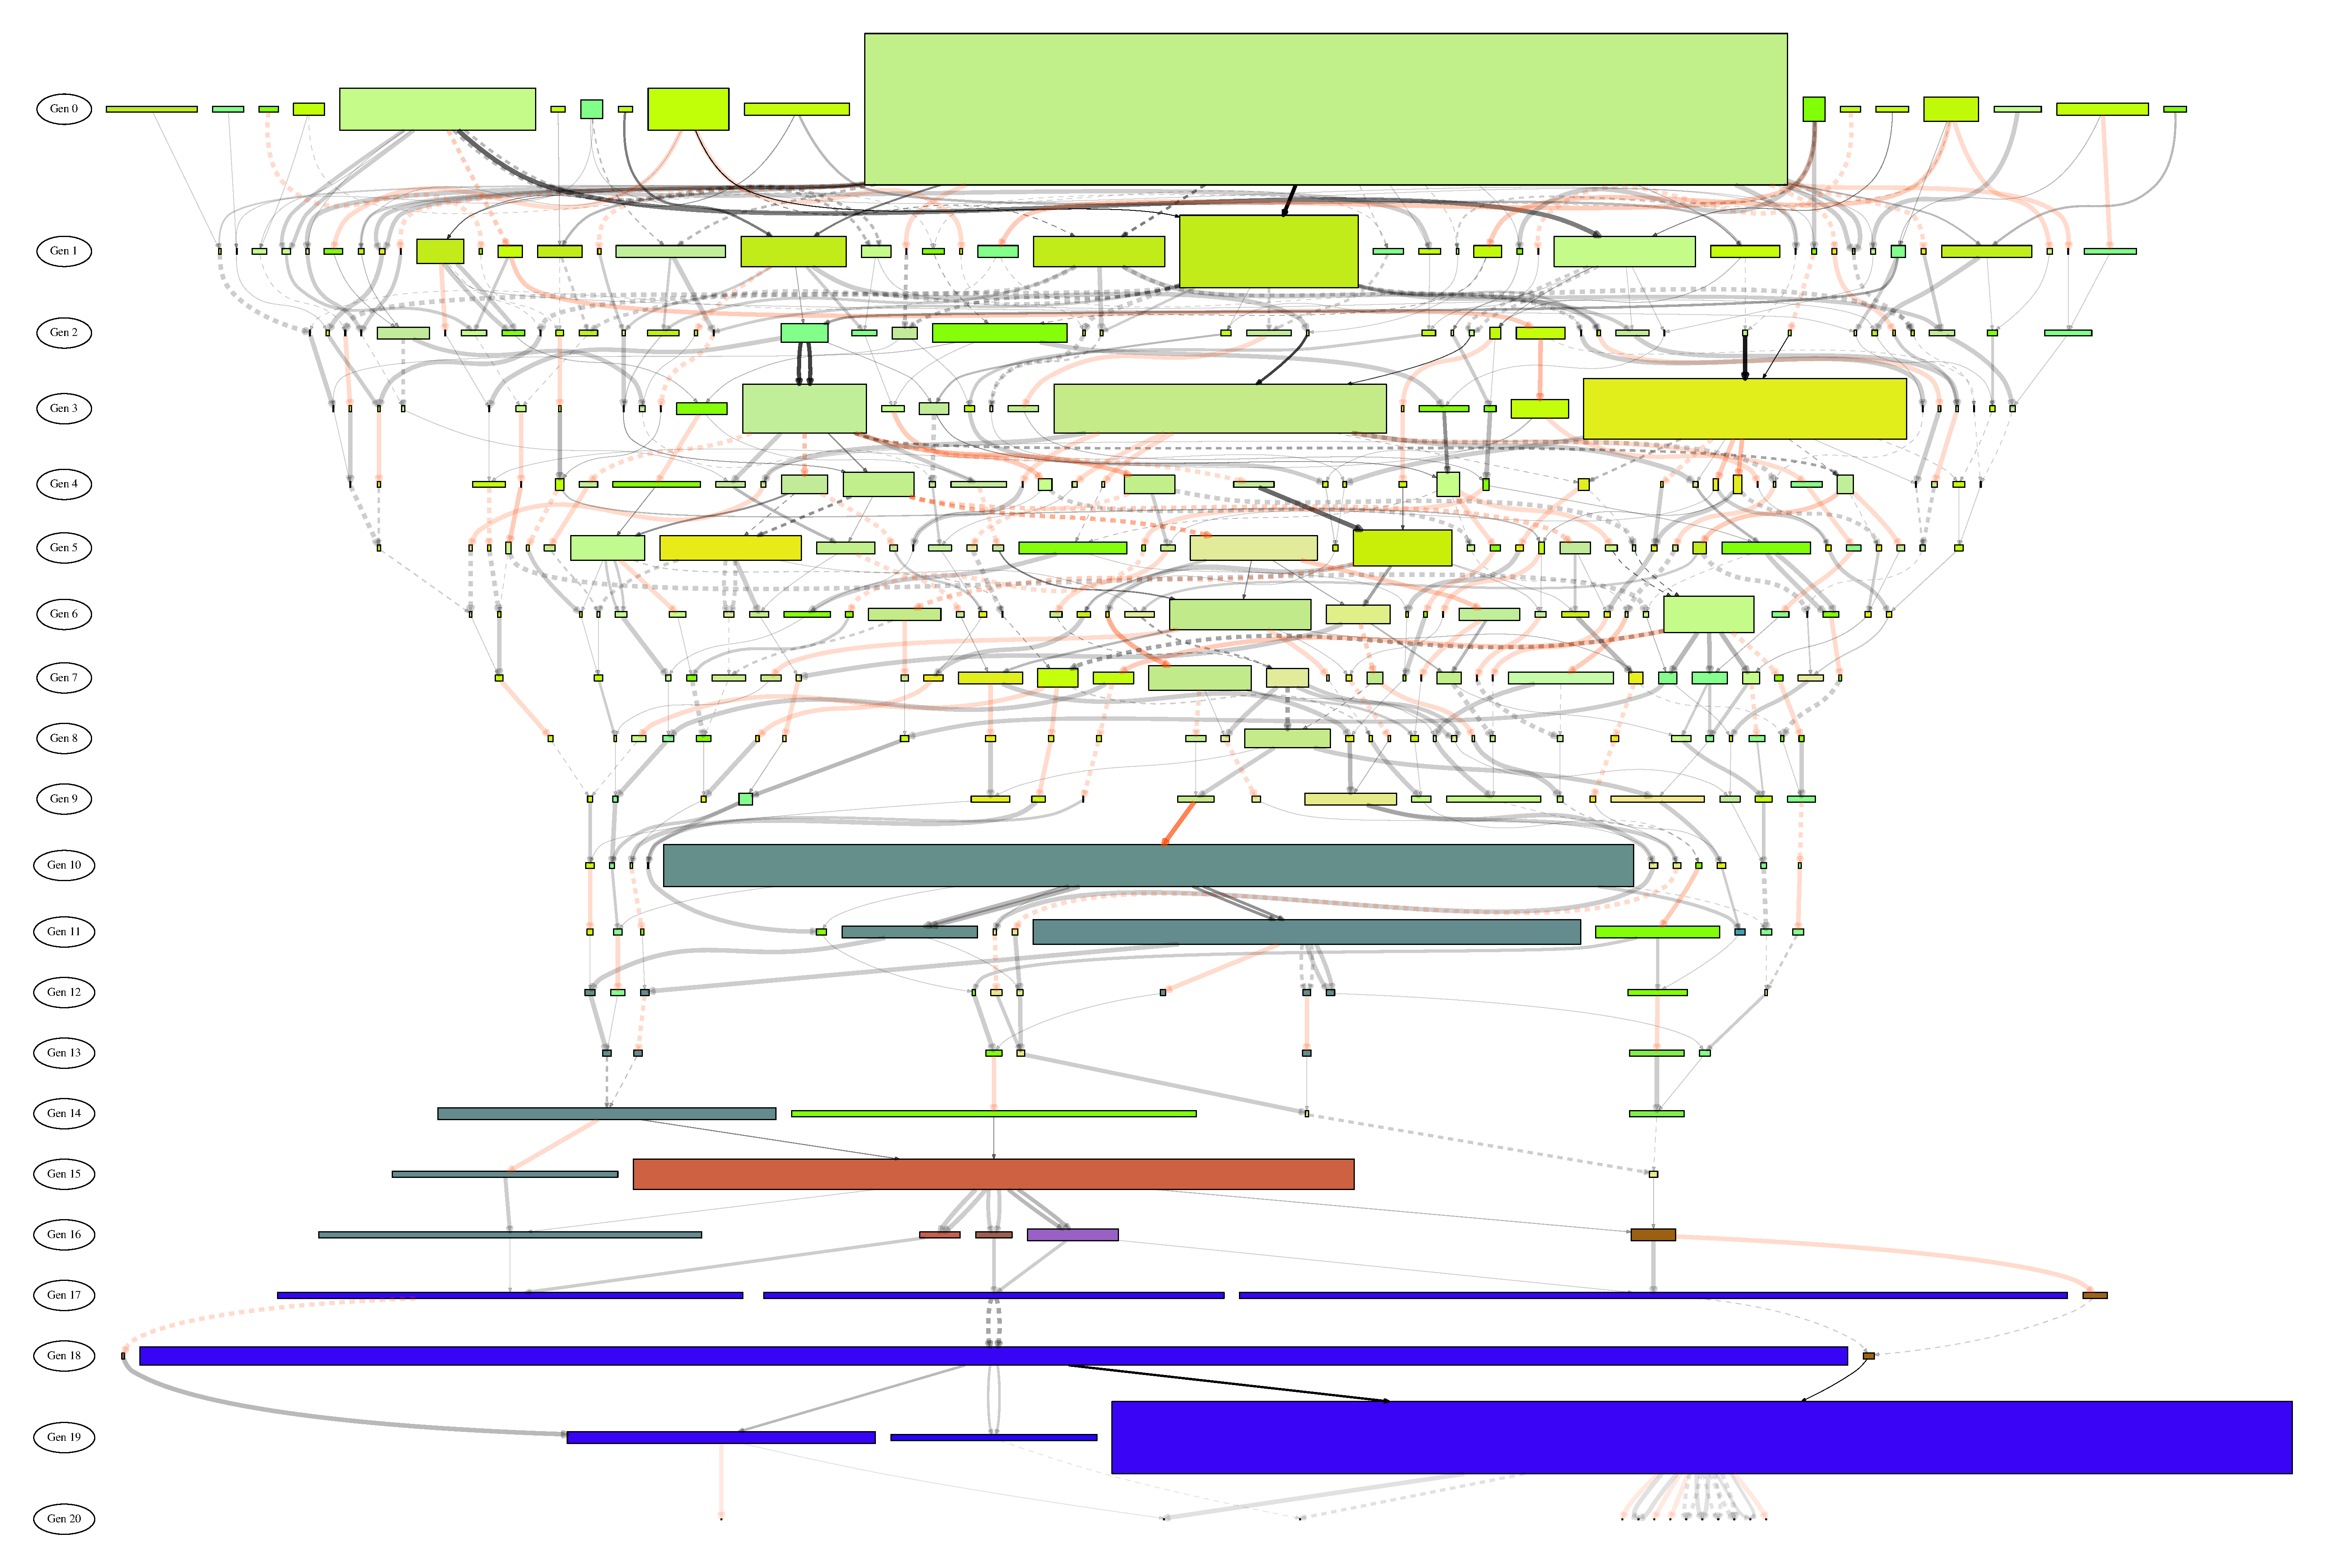
\includegraphics[width=1\linewidth]{../figures/run0_RBM_color_full_30000}
       % \begin{overprint}
       %   \onslide<2>
       %   Too many individuals!
       % \end{overprint}
   \end{frame}
   \begin{frame}
     \frametitle{Filtering - Simplified Ancestry}
     \centering
       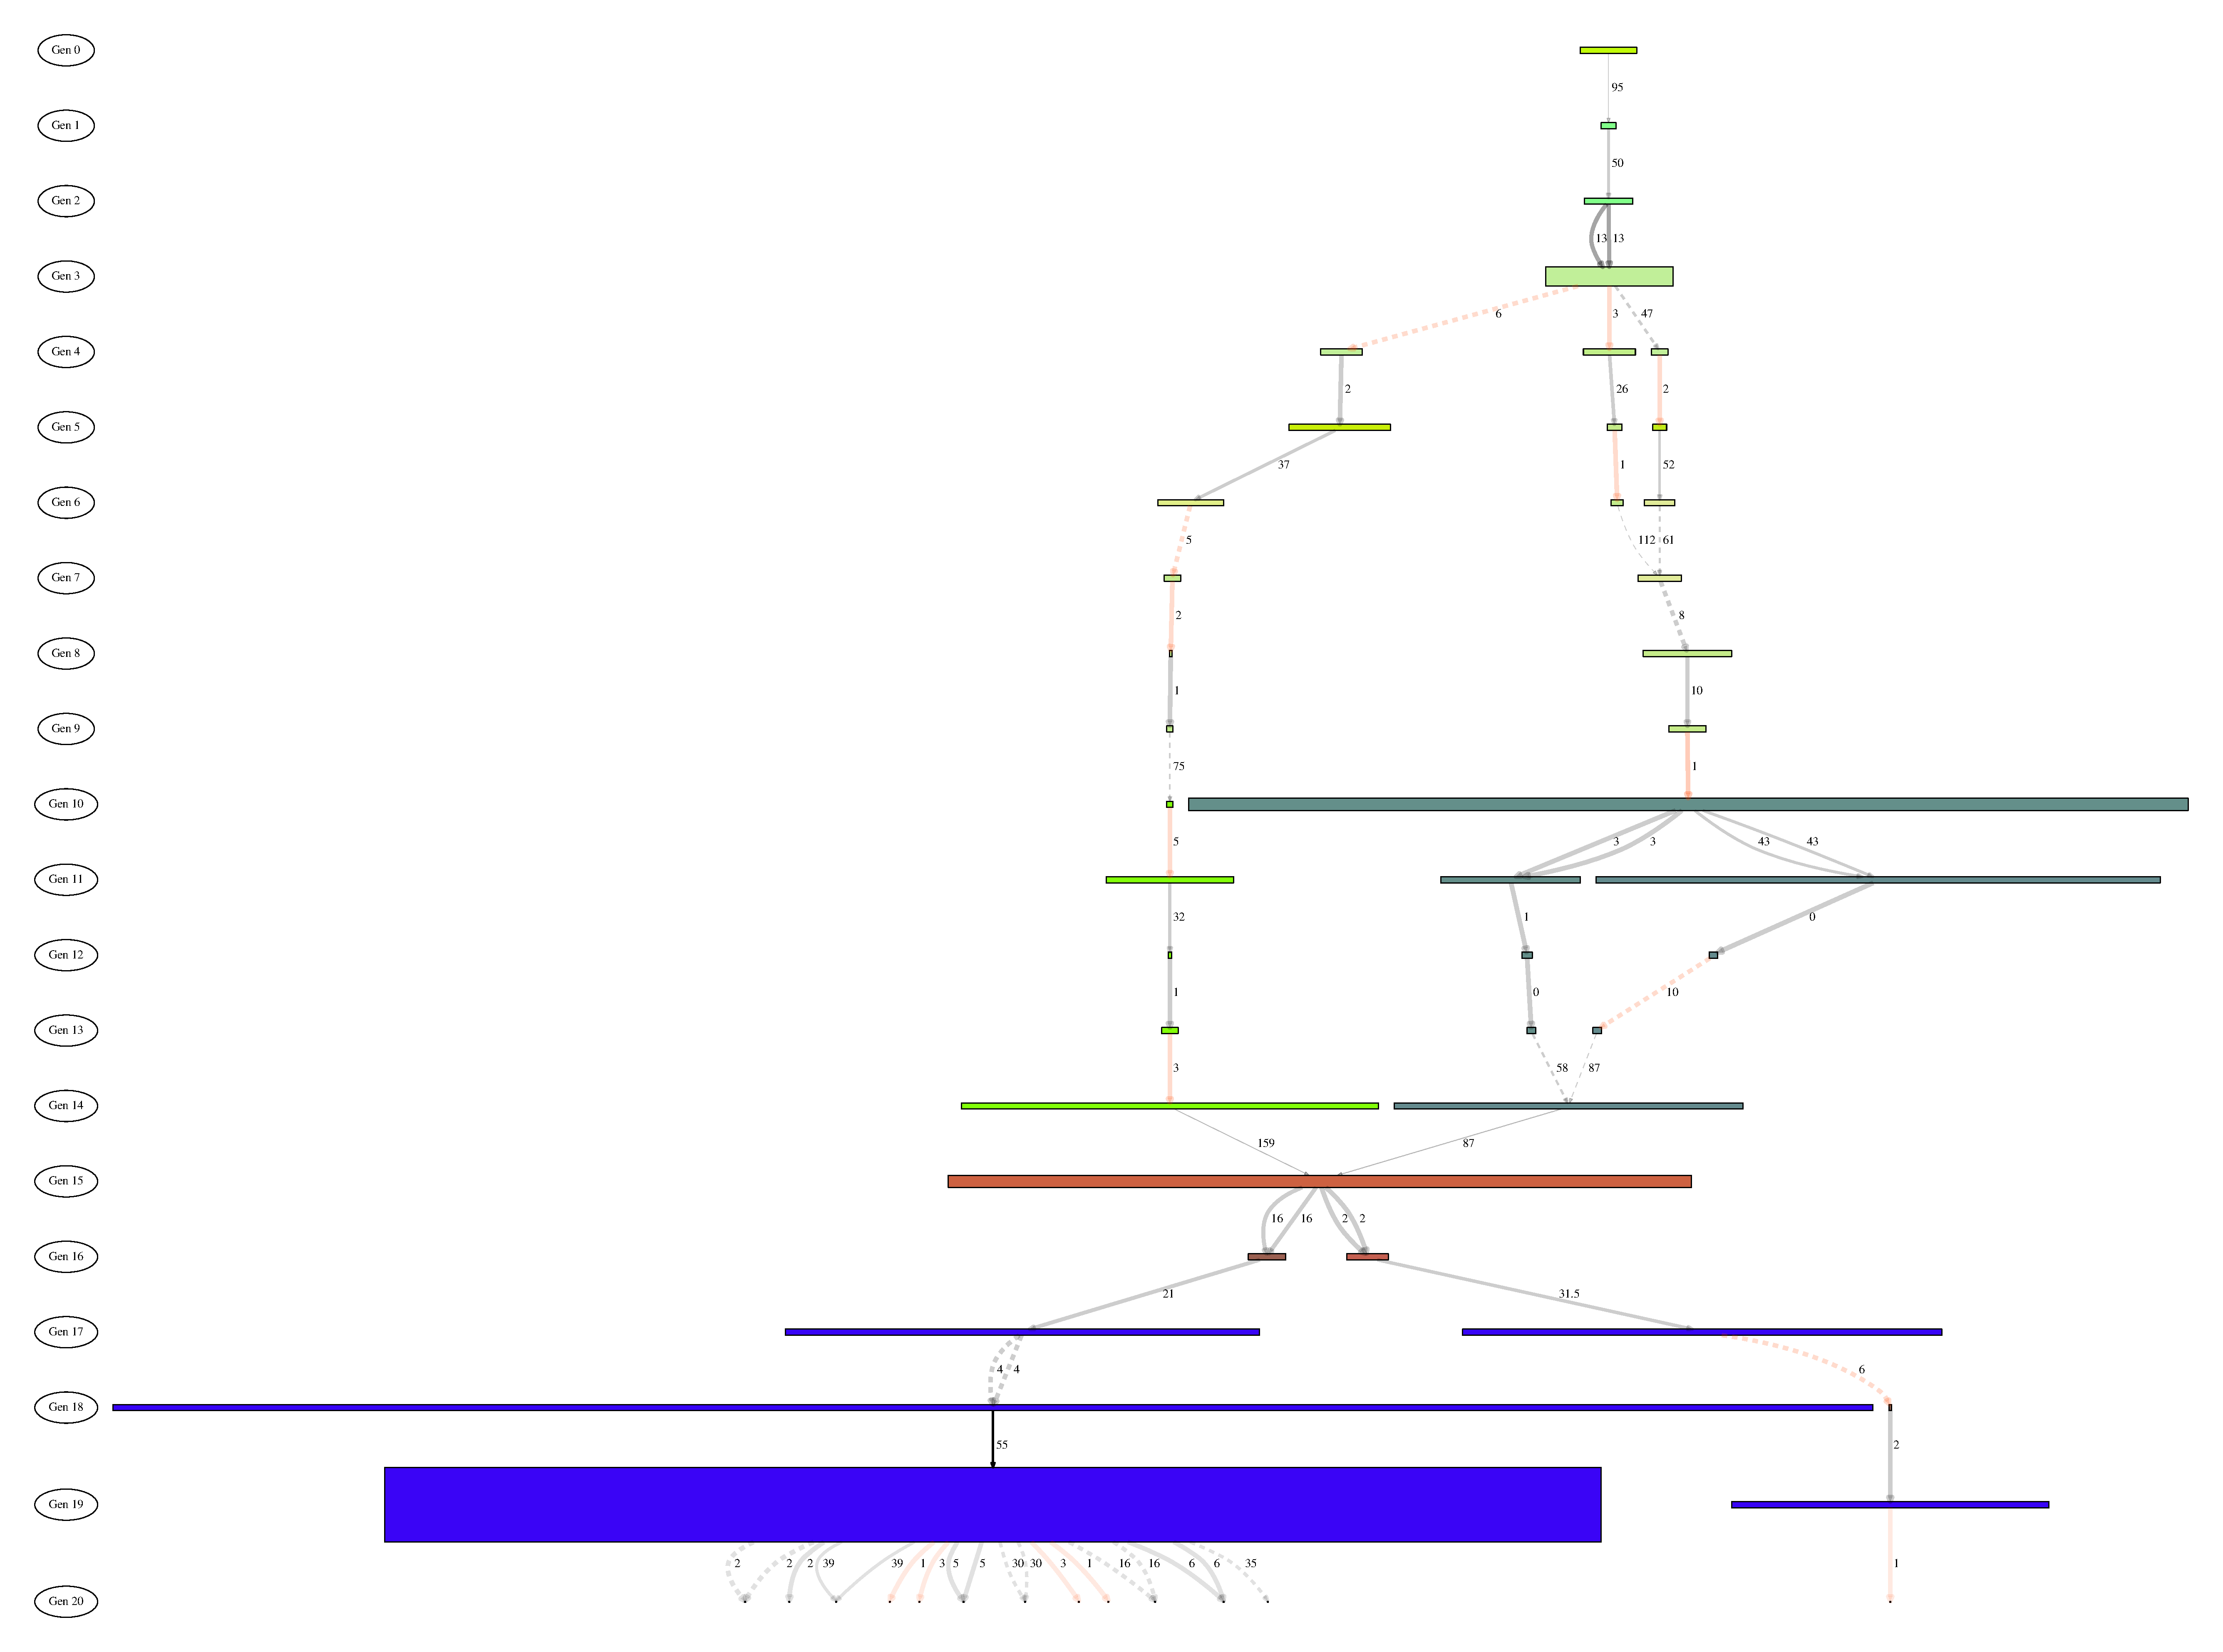
\includegraphics[width=1\linewidth]{../figures/run0_RBM_color_filtered_30000}
   \end{frame}

   % \begin{frame}
   %   \frametitle{Introducing the GPTP '16 Paper}
   %   \begin{overprint}
   %     \onslide<1>
   %     Where do winning individuals get their components?
   %   \end{overprint}
   %   % \begin{overprint}
   %   %    \onslide<2>
   %   %    asdf
   %   % \end{overprint}
   % \end{frame}

   \begin{frame}
     \frametitle{Analysing This Run}
     For all 40 individuals in the simplified family tree, we looked at...
     \begin{itemize}
     \item Genome
     \item Program
     \item Error vector
     \end{itemize}
     % \begin{itemize}
     % \item 40+ individual programs to analyze in the simplified ancestry
     20+ person-hours to summarize these individuals and their relationships
     % \end{itemize}
     % Compared genomes, the programs, and the test results. 
     % \begin{figure}
     %   \centering
     %   \def\svgwidth{0.25\linewidth}
     %   \input{genome2.pdf_tex}
     % \end{figure}
   \end{frame}

   \begin{frame}
     \frametitle{Findings}
     \begin{itemize}
     \item The genetic operators were used with the expected distribution...
     \item ...but alternation looked like mutation
     % \item Changes between generations were small
     \item Mutation played an important role
     \end{itemize}
   \end{frame} 
   
\section{This summer's work}

   \begin{frame}
     \frametitle{Motivation}
     \begin{itemize}
     \item These findings are only applicable to a specific run
     \item Filtering ancestry graphs by comparing genome similarity is time consuming and inexact
     \end{itemize}
   \end{frame}

\begin{frame}
  \frametitle{This summer's work}
  \begin{itemize}
  \item Modifying Clojush to report the source of each gene
  \item Designing a storage scheme
  \item Designing queries for the database
  \item Constructing a framework which automatically builds a report from this information
  \end{itemize}
  % Now that I've had a chance to play with the the DB system, would there be a
  % place where I could talk a little more about that? Is there anything that
  % I'd want to say?
\end{frame}

\begin{frame}
  Questions?
\end{frame}

\appendix

\begin{frame}[fragile]
  \frametitle{Example Push Genome}
\begin{verbatim}
[{:instruction 1 :close 0}
 {:instruction 2 :close 0}
 {:instruction integer_add :close 0}
 {:instruction 3 :close 0}
 {:instruction exec_if :close 0}
 {:instruction "equal" :close 0}
 {:instruction "not equal" :close 0}]
\end{verbatim}
\end{frame}
% \begin{frame}[fragile]
%   \frametitle{Example Push Program}
% \begin{overprint}
%   \onslide<1>
%   \begin{verbatim}
%   exec: (1 2 integer_add 3 integer_eq
%          exec_if  "not equal")
%    int: ()
%   bool: ()
% string: ()
%   \end{verbatim}
%   \onslide<2>
%   \begin{verbatim}
%   exec: (2 integer_add 3 integer_eq
%          exec_if "equal" "not equal")
%    int: (1)
%   bool: ()
% string: ()
%   \end{verbatim}
%   \onslide<3>
%    \begin{verbatim}
%   exec: (integer_add 3 integer_eq
%          exec_if "equal" "not equal")
%    int: (2 1)
%   bool: ()
% string: ()
% \end{verbatim}
%   \onslide<4>
%     \begin{verbatim}
%   exec: (3 integer_eq
%          exec_if "equal" "not equal")
%    int: (3)
%   bool: ()
% string: ()
% \end{verbatim}
%   \onslide<5>
%     \begin{verbatim}
%   exec: (integer_eq exec_if "equal" "not equal")
%    int: (3 3)
%   bool: ()
% string: ()
% \end{verbatim}
%   \onslide<6>
%      \begin{verbatim}
%   exec: (exec_if "equal" "not equal")
%    int: ()
%   bool: (true)
% string: ()
% \end{verbatim}
%   \onslide<7>
%      \begin{verbatim}
%   exec: ("equal")
%    int: ()
%   bool: ()
% string: ()
% \end{verbatim}
%   \onslide<8>
%      \begin{verbatim}
%   exec: ()
%    int: ()
%   bool: ()
% string: ("equal")
% \end{verbatim}
% \end{overprint}
% \end{frame}

\begin{frame}
  \frametitle{Lexicase Selection}
 TODO: have some details of how lexicase selection works
\end{frame}

\end{document}